\section{Конструкторский раздел}

\subsection{Проектирование базы данных}

На рисунке \ref{img:tables} представлена диаграмма проектируемой базы данных.

\begin{figure}[!h]
	\centering
	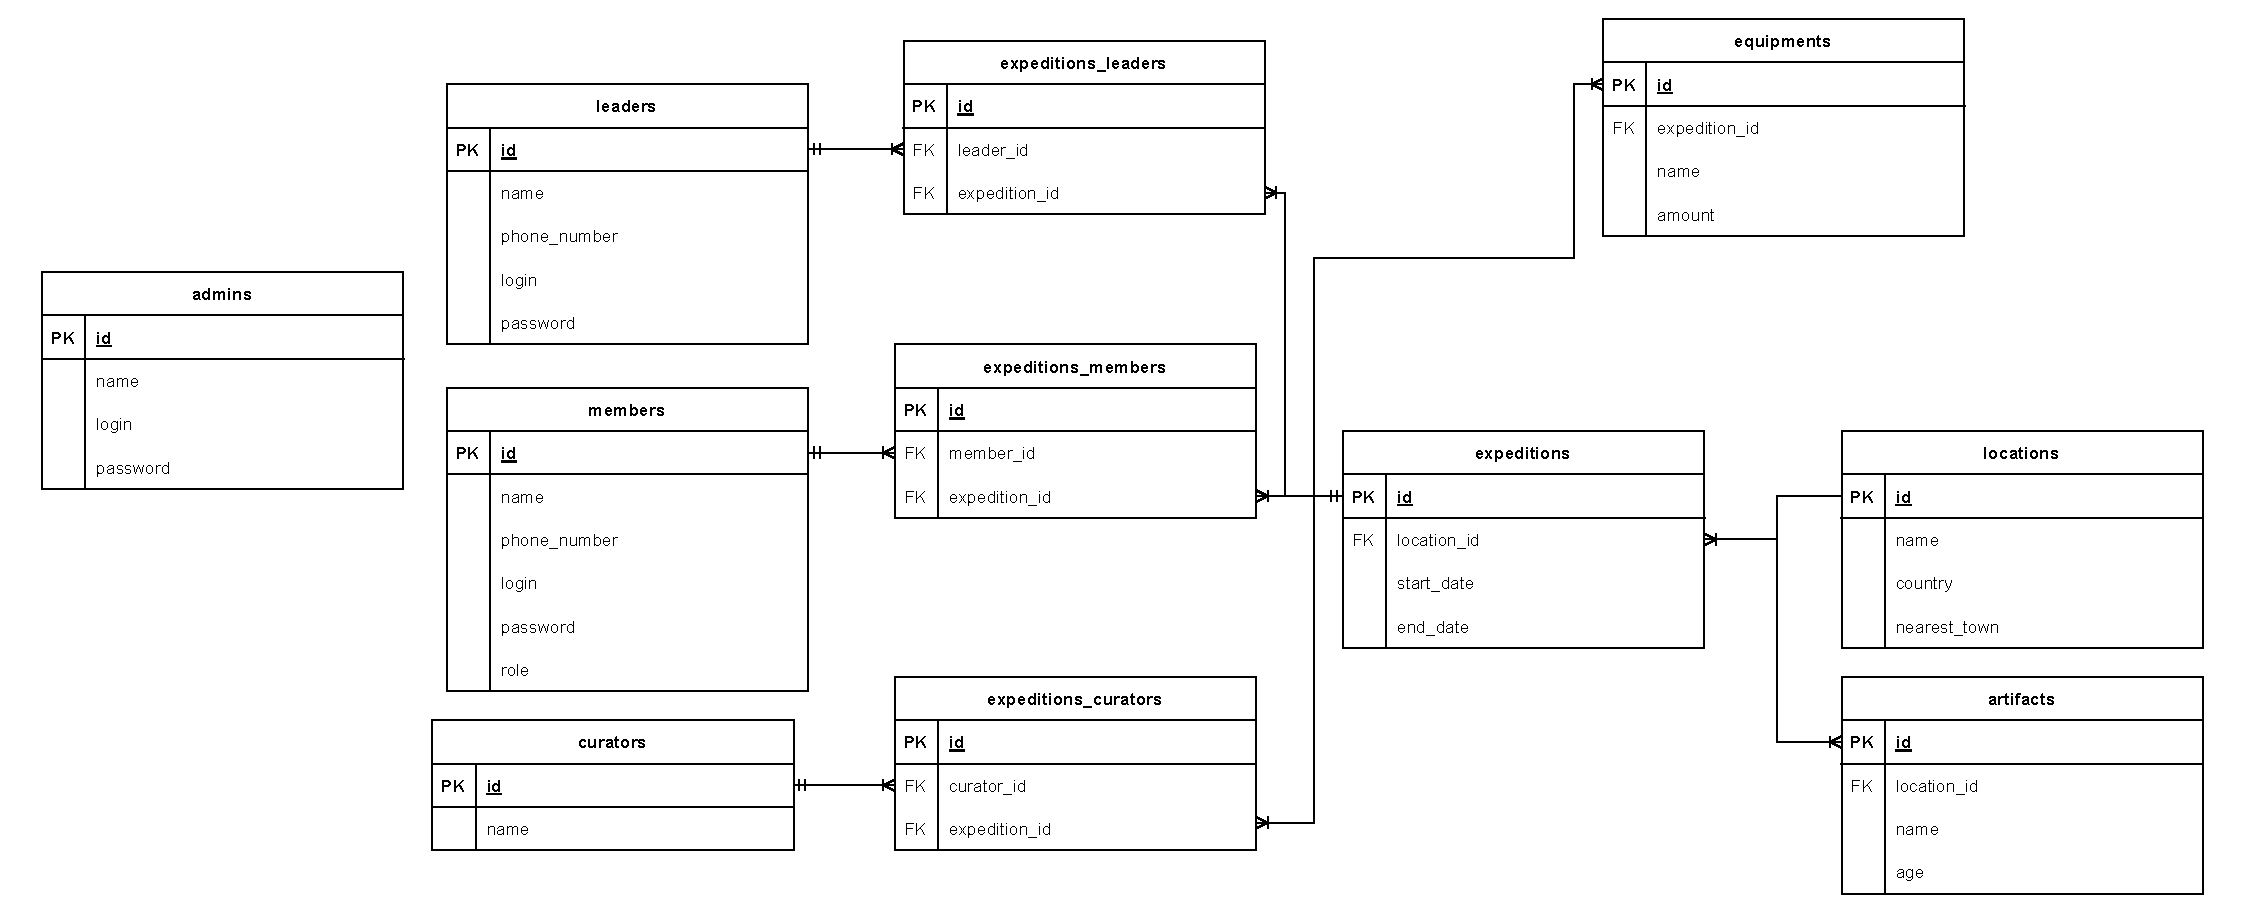
\includegraphics[width=\textwidth]{image/tables.pdf}
	\caption{Диаграмма базы данных}
	\label{img:tables}
\end{figure}

Таблица leaders хранит информацию о руководителях экспедиций и содержит следующие поля:

\begin{enumerate}[left=0.49cm, label=\arabic*.]
        \item id --- идентификатор руководителя, int;
	\item name --- имя руководителя, text;
	\item phone\_number --- номер телефона, text;
        \item login --- логин руководителя, text;
        \item password --- пароль, text.
\end{enumerate}

Таблица members хранит информацию об участниках экспедиций и содержит следующие поля:

\begin{enumerate}[left=0.49cm, label=\arabic*.]
        \item id --- идентификатор участника, int;
	\item name --- имя участника, text;
	\item phone\_number --- номер телефона, text;
        \item role --- роль участника в экспедиции, text;
        \item login --- логин участника, text;
        \item password --- пароль, text.
\end{enumerate}

Таблица admins хранит информацию об администраторах и содержит следующие поля:

\begin{enumerate}[left=0.49cm, label=\arabic*.]
        \item id --- идентификатор администратора, int;
	\item name --- имя администратора, text;
        \item login --- логин администратора, text;
        \item password --- пароль, text.
\end{enumerate}

Таблица curators хранит информацию о кураторах экспедиций и содержит следующие поля:

\begin{enumerate}[left=0.49cm, label=\arabic*.]
        \item id --- идентификатор куратора, int;
	\item name --- название, text.
\end{enumerate}

Таблица locations хранит информацию о местах проведения экспедиций и содержит следующие поля:

\begin{enumerate}[left=0.49cm, label=\arabic*.]
        \item id --- идентификатор локации, int;
	\item name --- название локации, text;
	\item country --- страна, text;
        \item nearest\_town --- ближайший населенный пункт, text.
\end{enumerate}

Таблица expeditions хранит информацию об экспедициях и содержит следующие поля:

\begin{enumerate}[left=0.49cm, label=\arabic*.]
        \item id --- идентификатор экспедиции, int;
	\item location\_id --- идентификатор места проведения экспедиции, int;
	\item start\_date --- дата начала экспедиции, date;
        \item end\_date --- дата окончания экспедиции, date.
\end{enumerate}

Таблица artifacts хранит информацию о найденных артефактах и содержит следующие поля:

\begin{enumerate}[left=0.49cm, label=\arabic*.]
        \item id --- идентификатор артефакта, int;
	\item location\_id --- идентификатор места обнаружения артефакта, int;
	\item name --- название артефакта, text;
        \item age --- возраст артефакта, int.
\end{enumerate}

Таблица equipments хранит информацию о снаряжении для экспедиции и содержит следующие поля:

\begin{enumerate}[left=0.49cm, label=\arabic*.]
        \item id --- идентификатор снаряжения, int;
	\item expedition\_id --- идентификатор экспедиции, int;
	\item name --- название снаряжение, text;
        \item amount --- количество снаряжения, int.
\end{enumerate}

Таблица expeditions\_leaders реализует связь <<многие-ко-многим>> таблиц expeditions и leaders и содержит следующие поля:

\begin{enumerate}[left=0.49cm, label=\arabic*.]
        \item id --- идентификатор записи, int;
        \item expedition\_id --- идентификатор экспедиции, int;
        \item leader\_id --- идентификатор руководителя, int.
\end{enumerate}

Таблица expeditions\_members реализует связь <<многие-ко-многим>> таблиц expeditions и members и содержит следующие поля:

\begin{enumerate}[left=0.49cm, label=\arabic*.]
        \item id --- идентификатор записи, int;
        \item expedition\_id --- идентификатор экспедиции, int;
        \item member\_id --- идентификатор участника, int.
\end{enumerate}

Таблица expeditions\_curators реализует связь <<многие-ко-многим>> таблиц expeditions и curators и содержит следующие поля:

\begin{enumerate}[left=0.49cm, label=\arabic*.]
        \item id --- идентификатор записи, int;
        \item expedition\_id --- идентификатор экспедиции, int;
        \item curator\_id --- идентификатор куратора, int.
\end{enumerate}



\subsection{Триггер базы данных}

Для добавления нового участника к экспедиции необходимо убедиться, что он не участвует в других экспедициях, пересекающихся по времени проведения с текущей. Для этого необходим триггер. При попытке добавления участника к экспедиции в  развязочной таблице для участников и экспедиций вызывается функция, схема алгоритма работы которой представлена на рисунке \ref{img:trigger}.

\begin{figure}[!h]
	\centering
	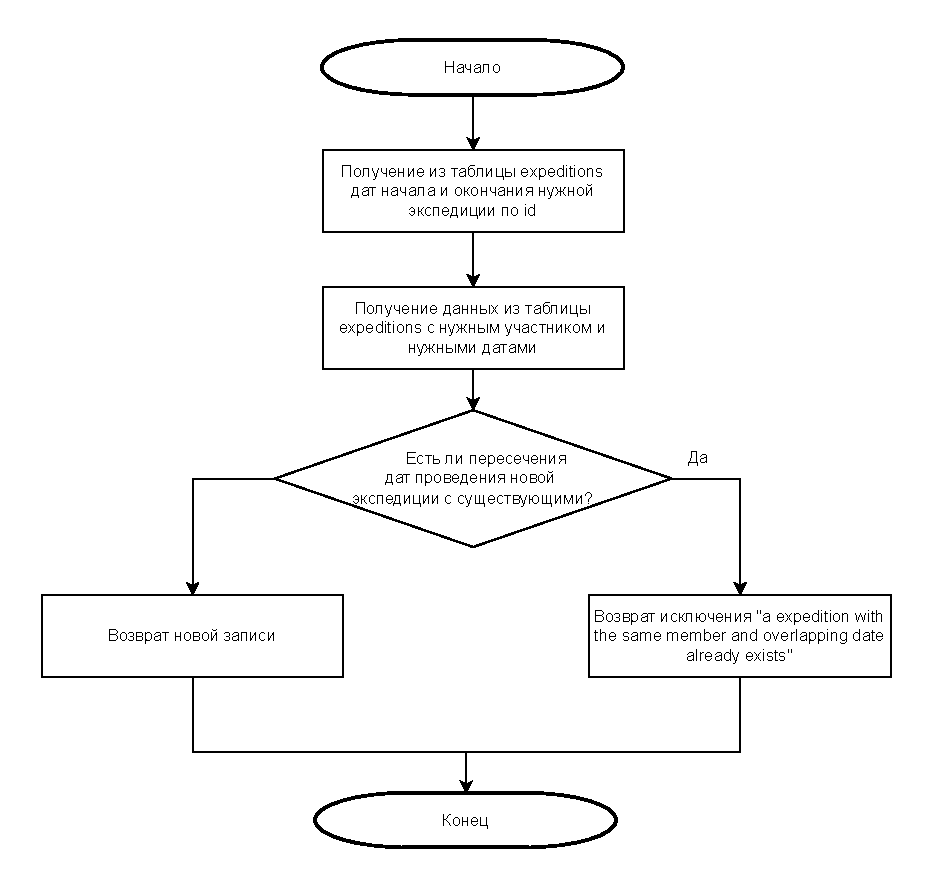
\includegraphics[width=\textwidth]{image/trigger.pdf}
	\caption{Схема алгоритма работы функции check\_expedition\_dates()}
	\label{img:trigger}
\end{figure}
\newpage


\subsection{Роли базы данных}

Разрабатываемая база данных имеет следующие роли.

\begin{enumerate}[left=0.49cm, label=\arabic*.]
	\item Участник --- права на выборку из таблиц expeditions, leaders, members, curators, locations, artifacts, equipments, expeditions\_leaders,\\ expeditions\_members, expeditions\_curators.
	\item Руководитель --- права на выборку из таблиц expeditions, leaders, members, curators, locations, artifacts, equipments, expeditions\_leaders,\\ expeditions\_members, expeditions\_curators; вставку в таблицы members,\\ expeditions, curators, locations, artifacts, equipments, expeditions\_members, expeditions\_curators; удаление из таблиц members, expeditions, curators, locations,  equipments, expeditions\_members, expeditions\_curators; изменение в таблице expeditions.
	\item Администратор --- права на все операции над всеми таблицами, создание таблиц и ролей.
\end{enumerate}


\subsection*{Вывод}
В данной части были описаны сущности, ролевая модель и функция базы данных.